\chapter{General Information}
\thispagestyle{fancy}


\section{Presentation of MS Innovative Smart System}

The \textbf{Internet of Things (IoT)} is expected to grow rapidly in the coming years. Often described as the fourth industrial revolution, IoT is a promising field, with over 20 billion smart devices projected to be connected by 2020. However, achieving this scale will involve overcoming several challenges at multiple levels. 

The \textbf{Innovative Smart Systems Master’s Program} aims to prepare young engineers to understand and tackle these challenges by developing innovative solutions. IoT systems consist of multiple layers, each with its own focus:

\begin{itemize}
    \item Perceptual Layer
    \item Network Layer
    \item Support Layer
    \item Application Layer
\end{itemize}

Each of these layers has specific challenges, addressed by different training units in the program:

\begin{itemize}
\item Designing smart devices: \textit{Smart Devices Training Unit}
\item Connecting devices: \textit{Communication Training Unit}
\item Processing data within the network: \textit{Data Processing Training Unit}
\item Providing services for network interaction and data access: \textit{Middleware and Services Training Unit}
\end{itemize}

This master’s program addresses these challenges through a variety of courses, bringing together students from diverse fields, including Electronics, Telecommunications, Computer Science, and Physics. By combining these skills, students can collaborate to solve the complex problems involved in developing IoT networks and systems.

\section{Curriculum}

\subsection{Student Profile}

\textbf{Personal information :} \\
Surname: VASSEUR.  \\
First name: Cyril.  \\
email: vasseu@insa-toulouse.fr.  \\

\subsection{Curriculum Vitae}

\begin{figure}[!ht]
    \centering
    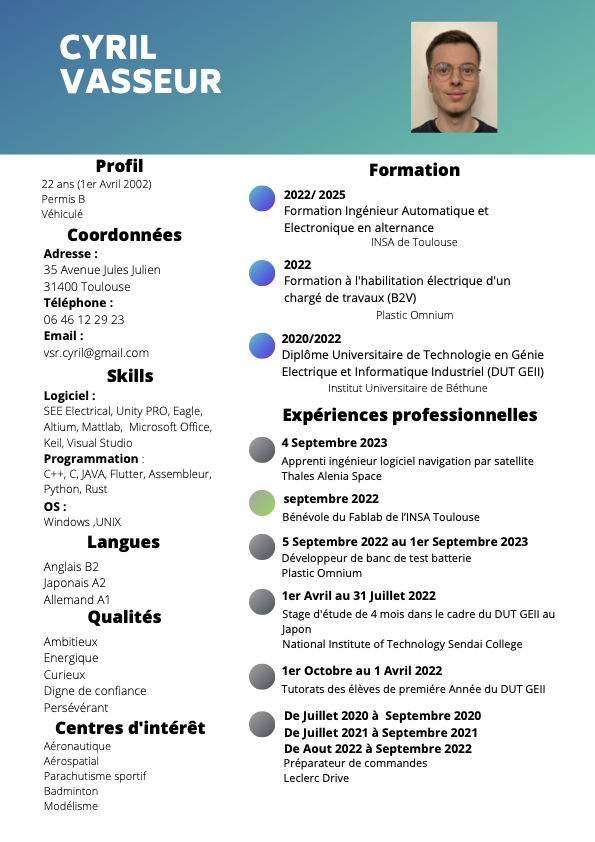
\includegraphics[width=0.6\textwidth]{image/CV_CYRIL VASSEUR.png}
    \caption{Curriculum Vitae}
    \label{fig:Curriculum Vitae}
\end{figure}

\vspace{1em} 

\newpage
\subsection{Background}

Before entering INSA for my third year of higher education, I completed a two-year technical diploma (DUT) in Electrical Engineering and Industrial Computing at IUT of Béthune. 
I then pursued an engineering degree at INSA Toulouse, where I began a Master’s in Automation and Electronics through an apprenticeship program. 
My first year was spent with Plastic Omnium, where I worked on developing a test bench for heavy vehicle batteries used in trains and trucks. 
For my second year, I moved to Thales Alenia Space, drawn by my interest in the space sector, where I became a software apprentice specializing in satellite navigation.
After completing my Master’s, I continued at Thales Alenia Space to pursue my second Master’s in Innovative Smart Systems (ISS).



\section{Training units}

Below, you can find the overview of the various courses completed in the ISS program.


\begin{figure}[!ht]
    \centering
    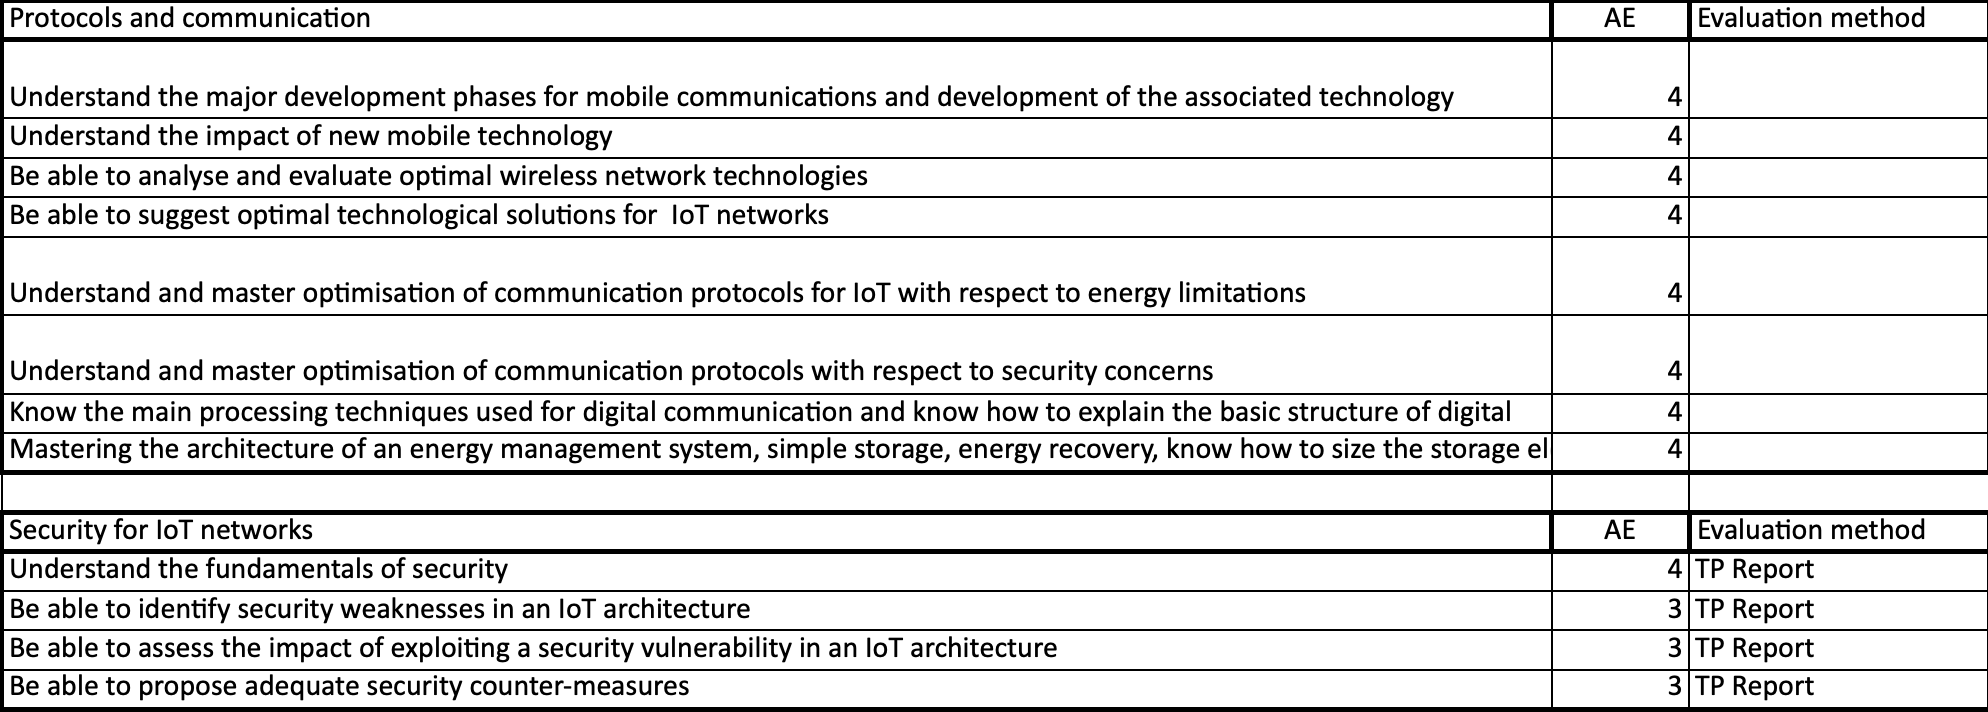
\includegraphics[width=0.8\textwidth]{image/Communication.png}
    \caption{Communication Unit}
    \label{fig:Communication}
\end{figure}
\begin{figure}[!ht]
    \centering
    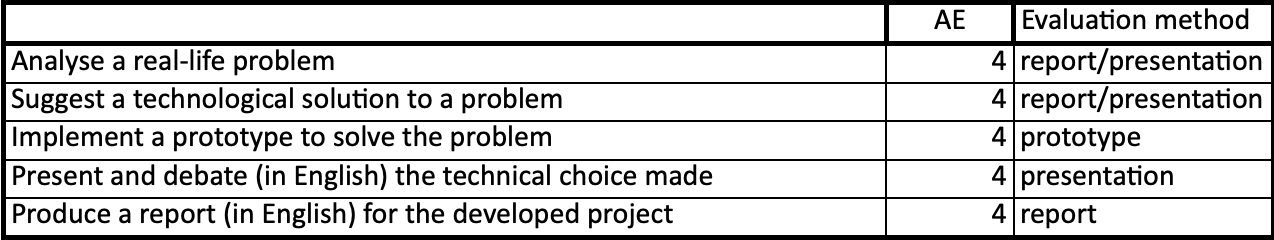
\includegraphics[width=0.8\textwidth]{image/Innovativ project.png}
    \caption{Innovative project Unit}
    \label{fig:Innovativ project}
\end{figure}
\begin{figure}[!ht]
    \centering
    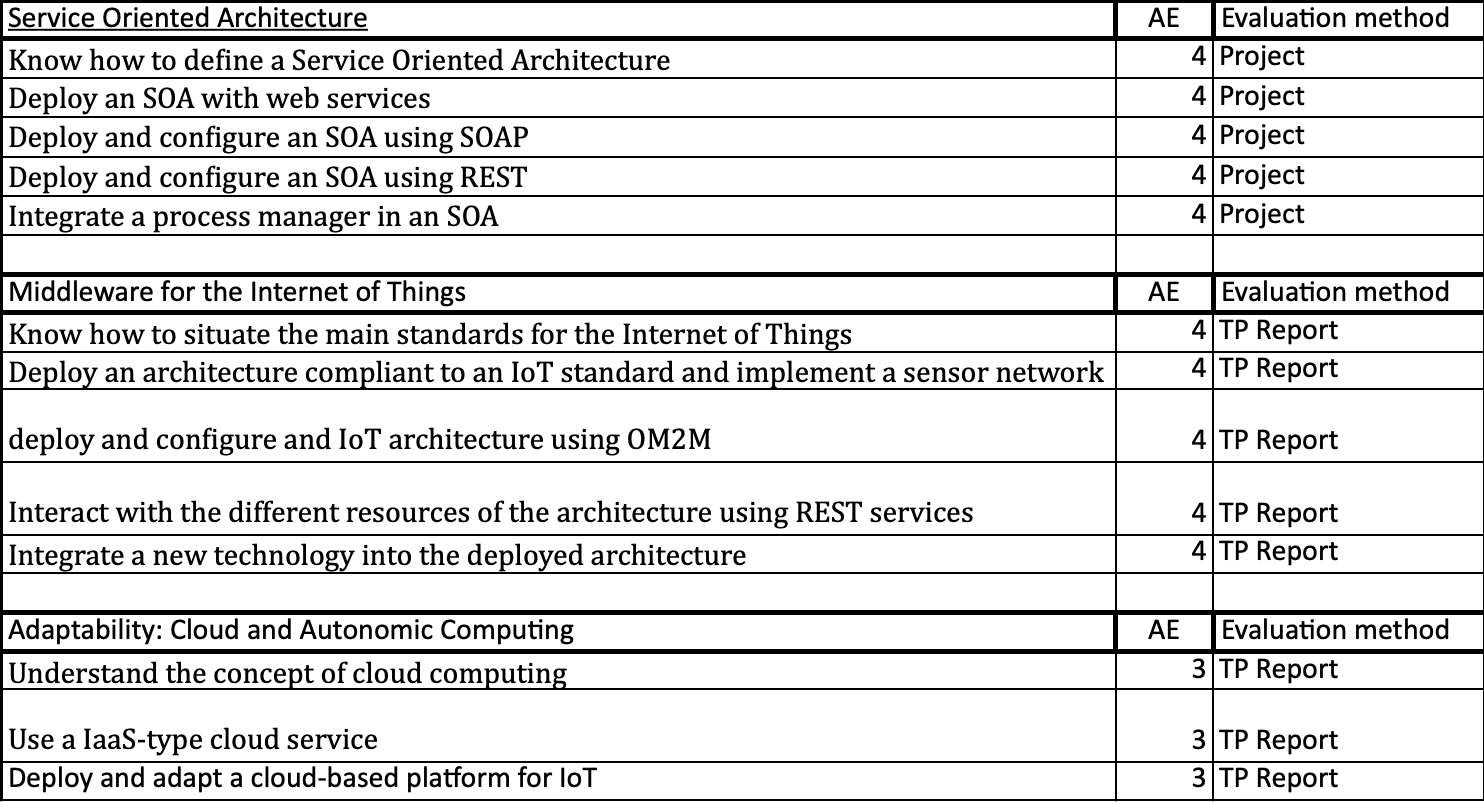
\includegraphics[width=0.8\textwidth]{image/Middleware and Service.png}
    \caption{Middleware and Service Unit}
    \label{fig:Middleware and Service}
\end{figure}
\begin{figure}[!ht]
    \centering
    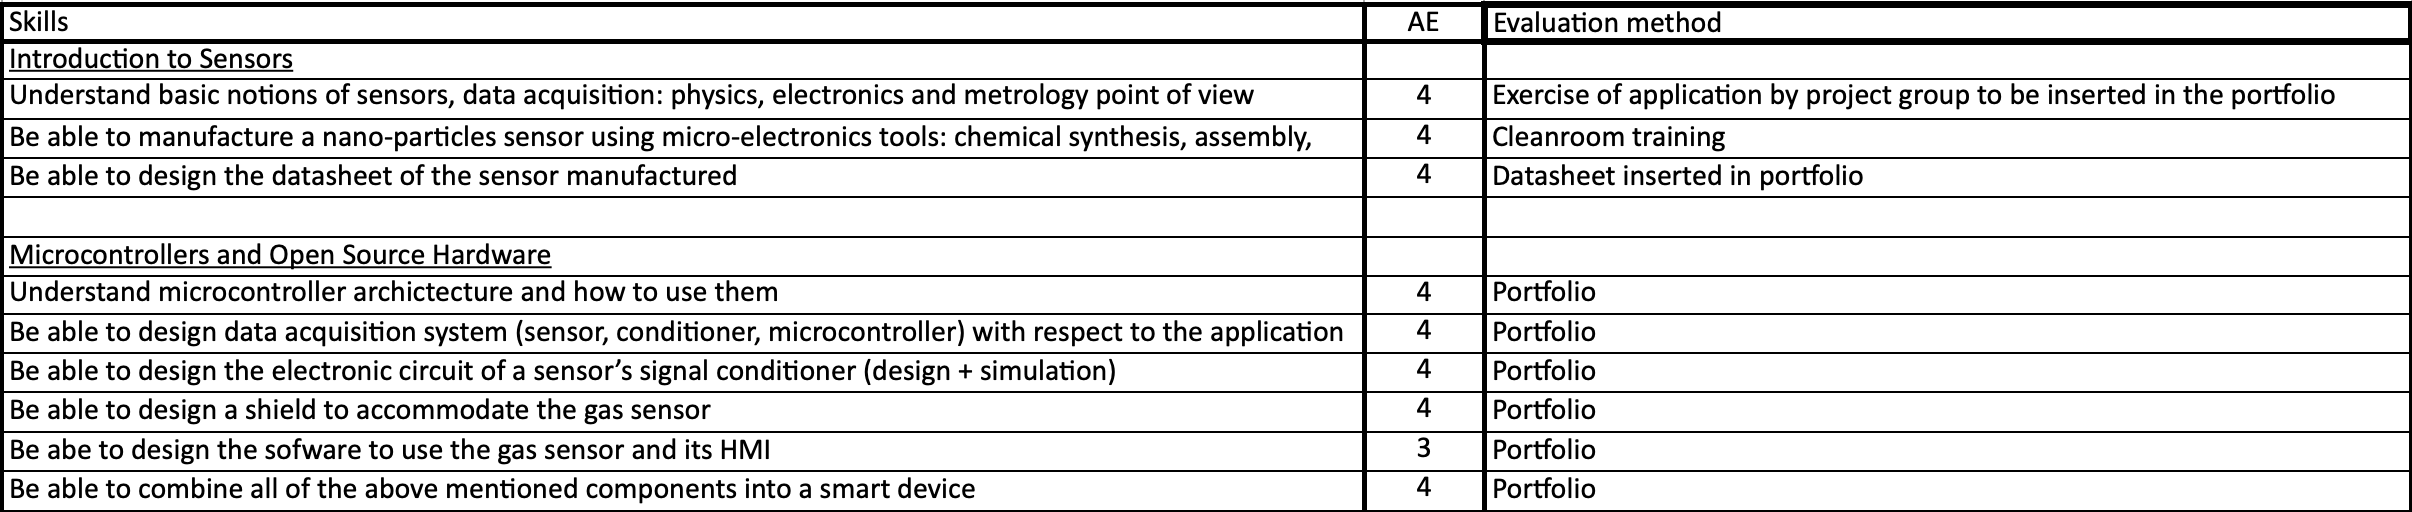
\includegraphics[width=0.8\textwidth]{image/Smart devices.png}
    \caption{Smart devices Unit}
    \label{fig:Smart devices}
\end{figure}
\newpage
\begin{figure}[!ht]
    \centering
    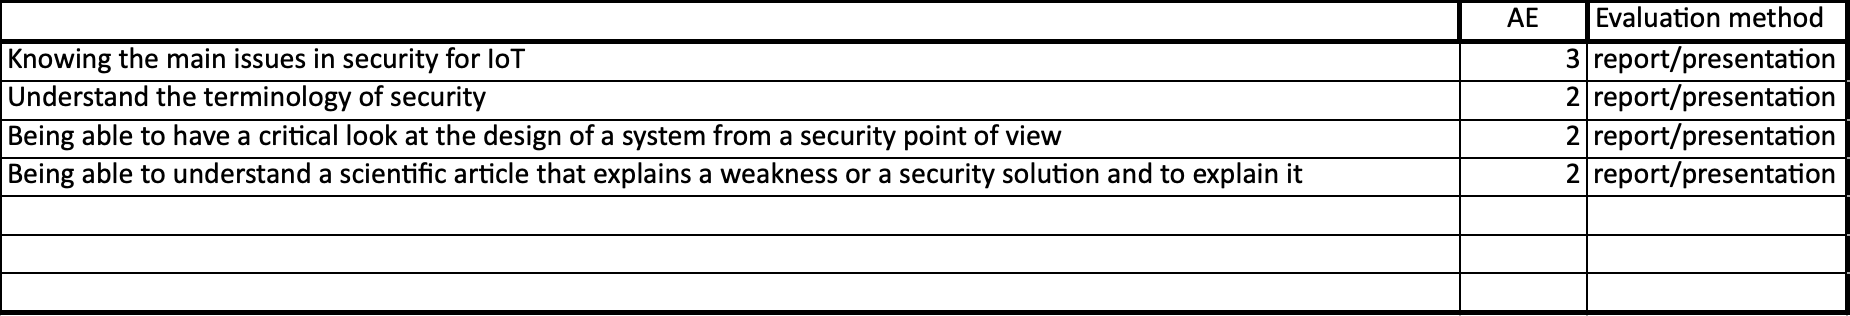
\includegraphics[width=0.8\textwidth]{image/Security.png}
    \caption{Security Unit}
    \label{fig:Security}
\end{figure}


\section{Apprenticeship}

\subsection{Why did I choose an apprenticeship}

During my years at INSA, I chose to pursue an apprenticeship, which is a way to combine academic studies with practical work in a company that finances both the training and the apprentice. This arrangement benefits the company by allowing it to train a future employee in advance so that they are operational immediately upon graduation.

In my first year at INSA, I was employed by Plastic Omnium. The department where I worked had recently been acquired, leading to significant changes in company policies. Consequently, most engineers who had transitioned into the new structure eventually decided to resign, including my former supervisor and my manager. After spending several months in this uncertain environment, I was offered the opportunity to leave the company to seek a more stable situation.

My decision strongly inclined toward Thales Alenia Space (TAS), primarily due to the nature of its activities and its reputation, which I heard about through word of mouth. I applied for several positions and was ultimately accepted for one as a Satellite Navigation Software Apprentice Engineer. I joined TAS in September 2023, allowing me to start the new academic year with peace of mind. I have remained with TAS since then, completing my final year of studies alongside my work with them.

\subsection{My sector of activities with Thales Alenia Space}

GNSS systems transmit information about the position and clock bias of each satellite, enabling users to locate themselves in the Earth-centered WGS 84 reference frame. However, the accuracy of GNSS navigation data is only guaranteed for a maximum of six hours, meaning there is a possibility that a satellite may broadcast erroneous positional information. While such errors usually do not affect non-critical systems, GNSS systems are not recommended for life-critical applications, such as guiding aircraft during airport approaches.

To address this limitation, the concept of an augmentation system was introduced. This system has two primary missions. The first is to calculate correction messages that allow aviation users relying on single-frequency GNSS signals to achieve precise localization. The second mission involves real-time monitoring of GNSS navigation data to detect anomalies and alert aviation users within a timeframe compatible with their flight phase.

Given that the requirements of civil aviation often cover extensive areas, using a geostationary satellite emerged as an obvious solution. Such an augmentation system is known as SBAS (Satellite-Based Augmentation System). An SBAS broadcasts a signal containing information about the reliability and accuracy of positioning signals from GPS and Galileo. This signal is designed to be processed by users without requiring major modifications.

The role of an SBAS is to analyze the various elements contributing to measurement errors and then broadcast dedicated augmentation messages containing corrections for each of these elements. User receivers recompose these corrections based on their geographic position, enhancing positioning accuracy and mitigating sources of error related to satellite clocks, positioning, and ionospheric effects.

\subsection{My mission and the final project}
 

My apprenticeship at Thales Alenia Space has been a defining and enriching experience, filled with diverse assignments and stimulating responsibilities. From the beginning, I benefited from a structured onboarding process that allowed me to master the tools and workflows essential to project execution.

Working in a collaborative environment with open spaces that encourage communication and quick problem resolution, I discovered the importance of high-performance equipment. For instance, I worked with a workstation equipped with 92 cores and 256 GB of RAM, which enabled me to run complex simulations, process large datasets, and maintain high levels of efficiency.

Agile methodology was at the heart of my activities, where I participated in daily meetings, sprint planning, and retrospectives. This approach allowed me to efficiently plan tasks and collaborate seamlessly with my team. It was particularly valuable for software development projects, where I used tools like Git to manage project lifecycles—from branch creation to pull requests—ensuring the quality of the produced code.

During this period, I used various programming languages, primarily Python and C. With Python, I developed analysis scripts and optimized existing tools to reduce execution times. I also worked on graphical representations to facilitate result interpretation and improve collaboration. In C, I designed features such as a stack trace to secure program execution, addressing complex issues related to compilation configurations, such as managing warnings and improving code flexibility.

A key mission was ensuring the quality of non-regression tests for SBAS scenarios. I updated outdated configurations and developed simulation scenarios covering diverse use cases. This involved managing massive datasets, ensuring traceability of changes, and maintaining reliable reference outputs. I also worked on enhancing scenario configurability, making the system more adaptable to new requirements.

Additionally, I contributed to resolving over 3,000 warnings during the compilation process—a challenge requiring a structured and collaborative approach. I developed automation tools to classify issues and proposed tailored solutions that balanced efficiency with compliance with company standards. These activities helped me develop a critical perspective and an analytical approach to complex technical problems.

In conclusion, my year at Thales Alenia Space allowed me to solidify my technical skills, immerse myself in a high-tech environment, and make meaningful contributions to the company’s projects. This experience motivates me to pursue a career in software engineering, tackling increasingly ambitious challenges.